%!TEX root = ../main.tex

\subsection{Normal component}\label{ss:normal_component}
% What?
This section discusses the parametrization of the normals. This section distinguishes between `fake' normals and `real' normals, in respectively section \ref{sss:method:normals:fakeNormals} and \ref{sss:method:normals:realNormals}. The fake normals are interpolated based on a quadratic patch, whereas the real normals are calculated based on the geometry of the point-normal triangle. 

It should be noted that just as the geometric component the normal component of the point-normal triangle is computed based on solely  the input primitive, i.e the vertex positions and their normals, as shown in \cref{fig:method:input_primitive}. 

\begin{figure}
	\centering
	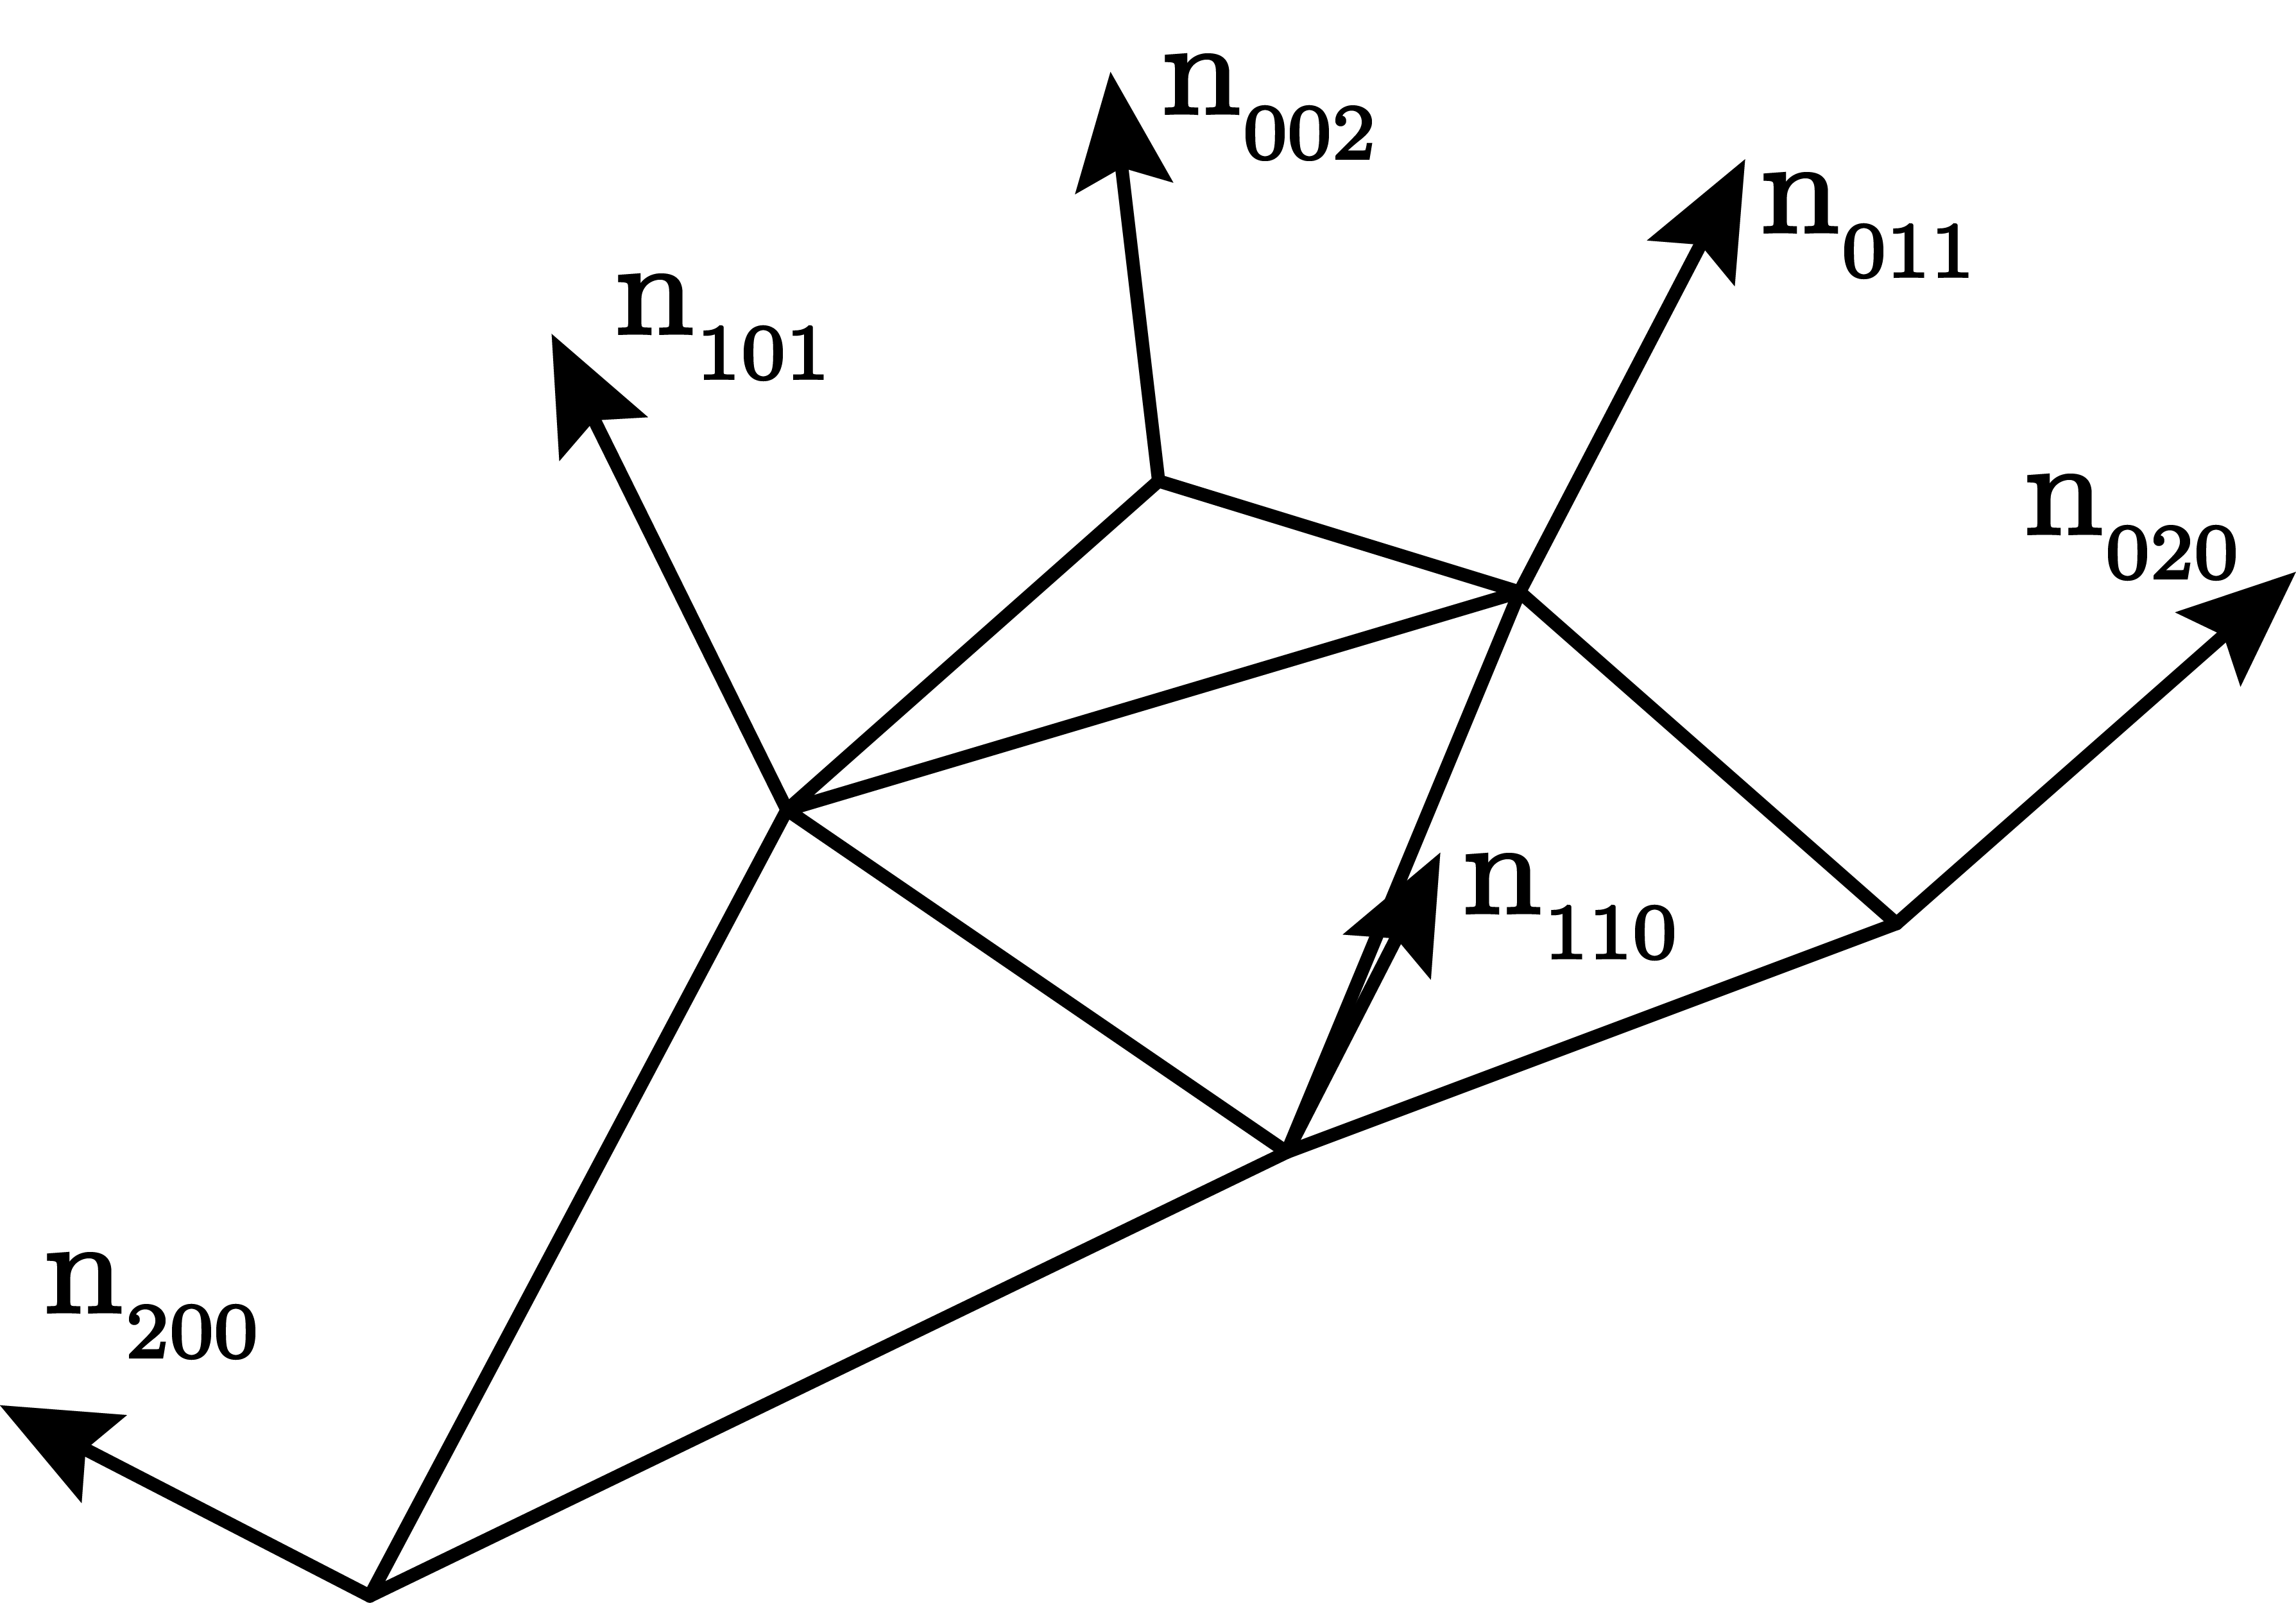
\includegraphics[width=0.45\textwidth]{./content/img/method/normals.png}
	\caption{The normal field of the point-normal triangle.}
	\label{fig:method:normal_field}
\end{figure}

\subsubsection{Fake normals}
\label{sss:method:normals:fakeNormals}
	\citeauthor{vlachos2001curved} defines the `fake' normals with quadratic function $n$:
	\begin{align}
	\noalign{$n: \quad R^2 \mapsto R^3,\quad$ for $w = 1 - u - v, \quad u, v, w \geq 0$}
	\begin{split}\label{eq:method:quadratic_normal_patch}
	    n(u,v) ={}& \sum_{i + j + k = 2} n_{ijk}u^i v^j w^k,\\
	      	   ={}& n_{200}w^2 + n_{020}u^2 + n_{002}v^2\\
	      	    {}& + n_{110}wu + n_{011}uv + n_{101}wv\\
	\end{split}
	\end{align}
	The coefficients of this quadratic `patch' are the normals shown in \cref{fig:method:normal_field}. The normals are computed for a point, halfway on every edge. Point-normal triangles use quadratically varying normals to be able capture the inflection points that are possible due to the cubic geometric component. 

	\Cref{fig:method:linear_vs_quadratically_varying} illustrates why one needs quadratic patches to capture these inflection points. 

	two cases: the top two images show a parabolic curve wGeehere both linear and quadratically varying normals perform the same. The more interesting case is the one illustrated by the two bottom images that show a cubic curve. We see that the linear varying normals do not capture the correct normal for this curve, but the quadratic varying normals do.

	% \begin{figure}
	% 	\plaatje{Splits met subcaptions voor beter verwijzen.}
	% 	\centering
	% 	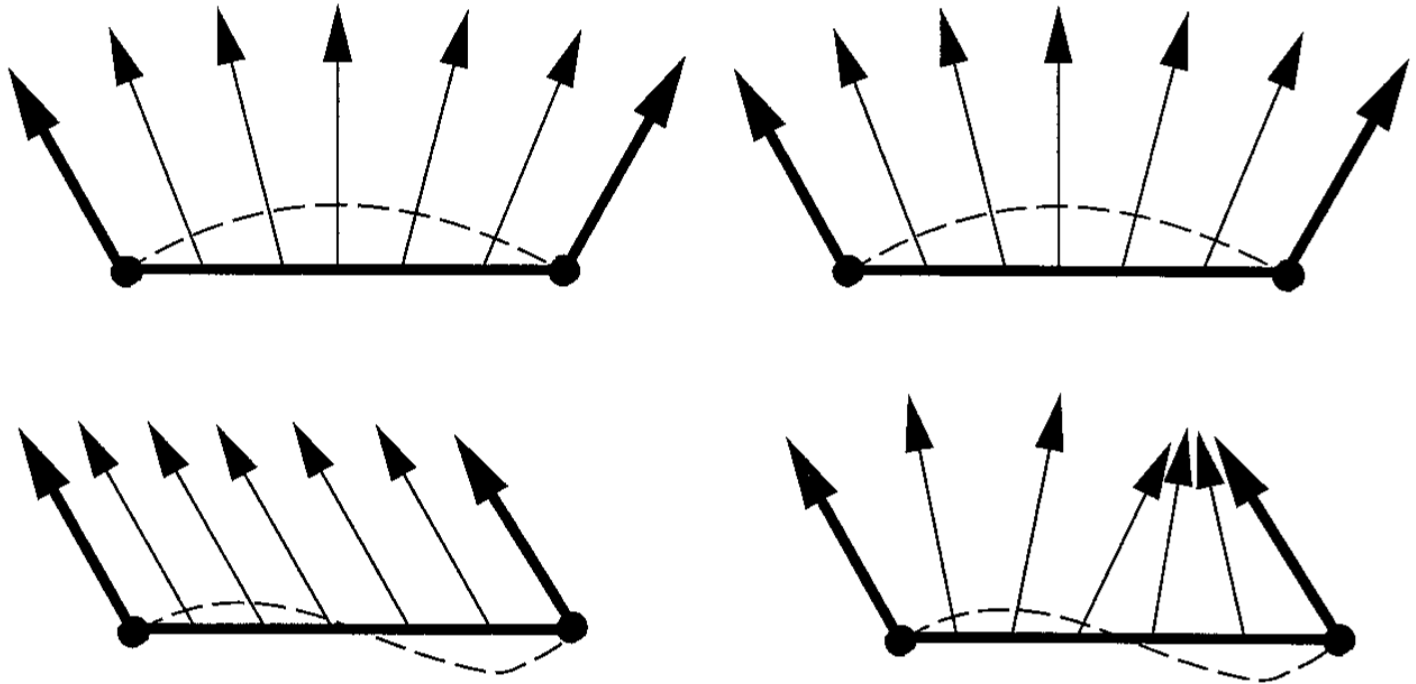
\includegraphics[width=0.45\textwidth]{./content/img/method/lin_vs_quad_varying_normals(inspiration).png}
	% 	\caption{The upper row shows a parabolic curve with linearly varying normals, on the left, and quadratically varying normals on the right. The lower row compares the normals of a cubic curve using linearly varying normals on the left and quadratically varying normals on the right. The illustration was taken form \textcite{van1997phong}.}
	% 	\label{fig:method:linear_vs_quadratically_varying}
	% \end{figure}


	\begin{figure}
		\centering
		\begin{subfigure}{\columnwidth}
			\centering
			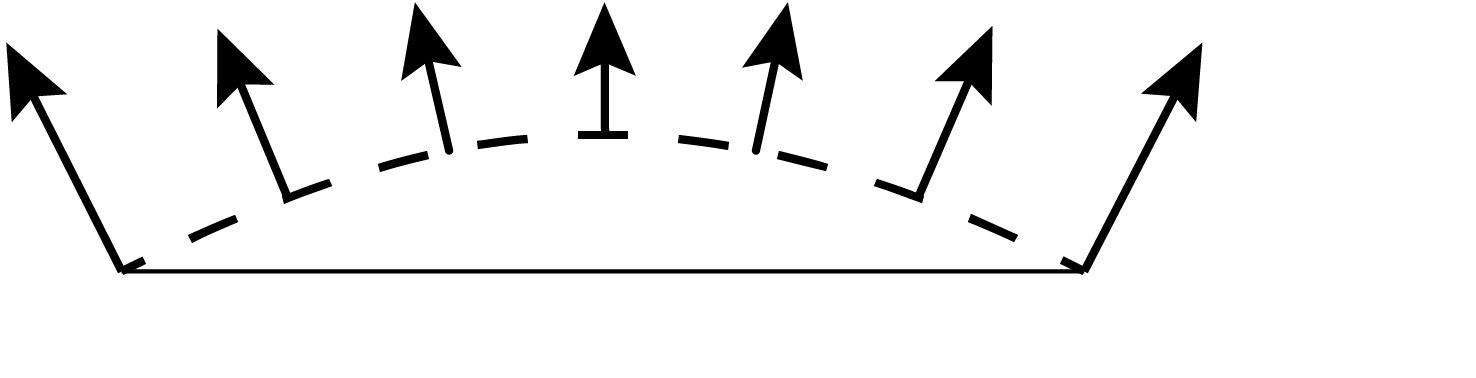
\includegraphics[width=\textwidth]{./content/img/method/linearVsQuadraticNormals_both.png}
			\caption{Vector averaging with either linear or quadratic over a curve without inflections.}
			\label{fig:method:normal:both}
		\end{subfigure}
		\begin{subfigure}{\columnwidth}
			\centering
			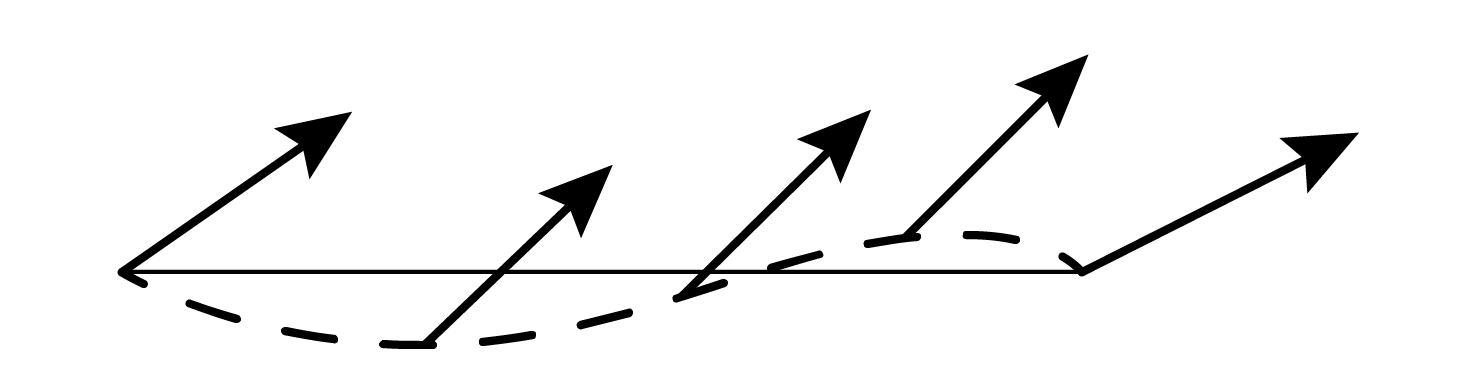
\includegraphics[width=\textwidth]{./content/img/method/linearVsQuadraticNormals_linear}
			\caption{Vector averaging with linear interpolation over a curve with an inflection.}
			\label{fig:method:normal:linear}
		\end{subfigure}	
		\begin{subfigure}{\columnwidth}
			\centering
			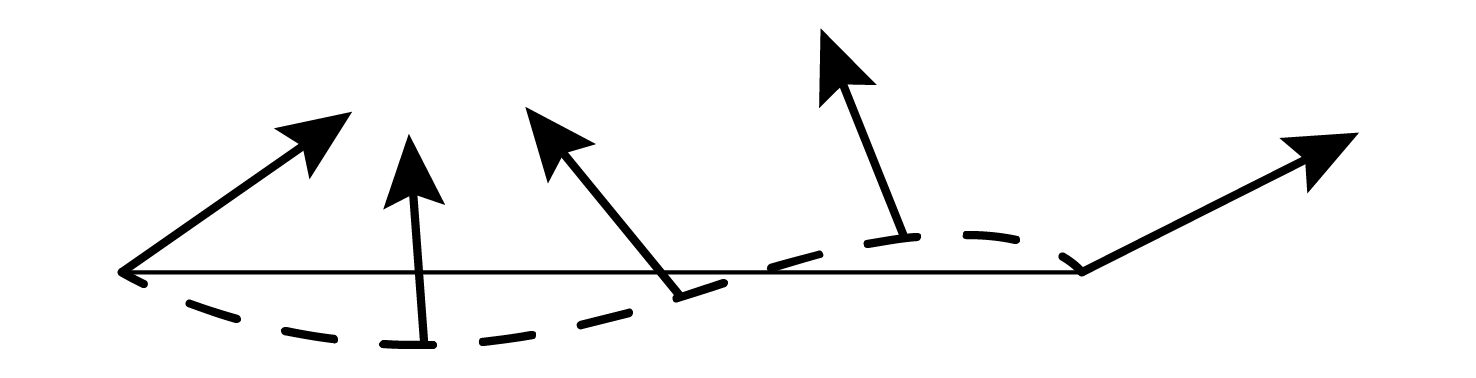
\includegraphics[width=\textwidth]{./content/img/method/linearVsQuadraticNormals_quadratic}
			\caption{Vector averaging with quadratic interpolation over a curve with an inflection.}
			\label{fig:method:normal:quadratic}
		\end{subfigure}			
		\caption{Some examples of normal vector averaging over an edge. The dashed lines indicate the profile of the surface that should be approximated. The normals of a curves without inflections are correctly approximated by both linear and quadratic interpolation, see \cref{fig:method:normal:both}. The normals of a curve with inflections are incorrectly approximated with \subref{fig:method:normal:linear} linear interpolation and correctly with \subref{fig:method:normal:quadratic} interpolation. Image \subref{fig:method:normal:both} was adapted from \cite{van1997phong}, \subref{fig:method:normal:linear} and \subref{fig:method:normal:quadratic} from \cite{vlachos2001curved}.}
		\label{fig:method:normal}
	\end{figure}

	\todo[inline]{Discuss parametrization of `quadratic' patch}

	Using the function $n$, see \eqref{eq:method:quadratic_normal_patch}, the normal of any point parametrized by the barycentric coordinates $u$ and $v$ can be calculated. To do this we first need to define a control net. We consider two different types of coefficients: the vertex normals, $n_{200}$, $n_{020}$, and $n_{002}$; and the edge normals, $n_{110}$, $n_{011}$, and $n_{101}$. 
	\todo[inline]{Discuss the construction of the control points for the `quadratic' patch}

\subsubsection{Real normals}
\label{sss:method:normals:realNormals}
		\todo[inline]{Discuss how to compute the real normals given the geometric component}
		The real normals are computed based on the geometric component of the point-normal triangle. This is done by taking the cross product of the the partial derivatives with respect to $u$ and $v$. 

		\todo[inline]{Expand explanation, add math}